%
% This is the LaTeX template file for lecture notes for CS294-8,
% Computational Biology for Computer Scientists.  When preparing 
% LaTeX notes for this class, please use this template.
%
% To familiarize yourself with this template, the body contains
% some examples of its use.  Look them over.  Then you can
% run LaTeX on this file.  After you have LaTeXed this file then
% you can look over the result either by printing it out with
% dvips or using xdvi.
%
% This template is based on the template for Prof. Sinclair's CS 270.

\documentclass[twoside]{article}
\usepackage{graphics}
\usepackage{amsfonts}
\usepackage{tikz}
\usepackage{amsmath}

\usetikzlibrary{chains,fit,shapes}
\setlength{\oddsidemargin}{0.25 in}
\setlength{\evensidemargin}{-0.25 in}
\setlength{\topmargin}{-0.6 in}
\setlength{\textwidth}{6.5 in}
\setlength{\textheight}{8.5 in}
\setlength{\headsep}{0.75 in}
\setlength{\parindent}{0 in}
\setlength{\parskip}{0.1 in}

%
% The following commands set up the lecnum (lecture number)
% counter and make various numbering schemes work relative
% to the lecture number.
%
\newcounter{lecnum}
\renewcommand{\thepage}{\thelecnum-\arabic{page}}
\renewcommand{\thesection}{\thelecnum.\arabic{section}}
\renewcommand{\theequation}{\thelecnum.\arabic{equation}}
\renewcommand{\thefigure}{\thelecnum.\arabic{figure}}
\renewcommand{\thetable}{\thelecnum.\arabic{table}}

%
% The following macro is used to generate the header.
%
\newcommand{\chno}[4]{
   \pagestyle{headings}
   \thispagestyle{plain}
   \newpage
   \setcounter{lecnum}{#1}
   \setcounter{page}{1}
   \noindent
   \begin{center}
   \framebox{
      \vbox{\vspace{2mm}
    \hbox to 6.28in { {\bf CIS 511: Theory of Computation
                        \hfill Jan 24, 2017} }
       \vspace{4mm}
       \hbox to 6.28in { {\Large \hfill Lecture #1: #2  \hfill} }
       \vspace{2mm}
       \hbox to 6.28in { {\it Professor #3 \hfill #4} }
      \vspace{2mm}}
   }
   \end{center}
   \markboth{Lecture #1: #2}{Lecture #1: #2}
   {\bf NB}: {\it These notes are from CIS511 at Penn. The course followed Michael Sipser's \textit{Introduction to the Theory of Computation (3ed)} text.}
   \vspace*{4mm}
}

%
% Convention for citations is authors' initials followed by the year.
% For example, to cite a paper by Leighton and Maggs you would type
% \cite{LM89}, and to cite a paper by Strassen you would type \cite{S69}.
% (To avoid bibliography problems, for now we redefine the \cite command.)
% Also commands that create a suitable format for the reference list.
\renewcommand{\cite}[1]{[#1]}
\def\beginrefs{\begin{list}%
        {[\arabic{equation}]}{\usecounter{equation}
         \setlength{\leftmargin}{2.0truecm}\setlength{\labelsep}{0.4truecm}%
         \setlength{\labelwidth}{1.6truecm}}}
\def\endrefs{\end{list}}
\def\bibentry#1{\item[\hbox{[#1]}]}

%Use this command for a figure; it puts a figure in wherever you want it.
%usage: \fig{NUMBER}{SPACE-IN-INCHES}{CAPTION}
\newcommand{\fig}[3]{
			\vspace{#2}
			\begin{center}
			Figure \thelecnum.#1:~#3
			\end{center}
	}
% Use these for theorems, lemmas, proofs, etc.
\newtheorem{theorem}{Theorem}[lecnum]
\newtheorem{lemma}[theorem]{Lemma}
\newtheorem{proposition}[theorem]{Proposition}
\newtheorem{claim}[theorem]{Claim}
\newtheorem{corollary}[theorem]{Corollary}
\newtheorem{definition}[theorem]{Definition}
\newenvironment{proof}{{\bf Proof:}}{\hfill\rule{2mm}{2mm}}

% **** IF YOU WANT TO DEFINE ADDITIONAL MACROS FOR YOURSELF, PUT THEM HERE:

\begin{document}
%FILL IN THE RIGHT INFO.
%\lecture{**LECTURE-NUMBER**}{**DATE**}{**LECTURER**}{**SCRIBE**}
\chno{4}{More Turing Machines}{Sampath Kannan}{Zach Schutzman}
%\footnotetext{These notes are partially based on those of Nigel Mansell.}

% **** YOUR NOTES GO HERE:

% Some general latex examples and examples making use of the
% macros follow.  
%**** IN GENERAL, BE BRIEF. LONG SCRIBE NOTES, NO MATTER HOW WELL WRITTEN,
%**** ARE NEVER READ BY ANYBODY.



\section*{Turing Machines}

Let $B=\{w\#w | w\in\Sigma^*\}$.  Here is a TM to accept this language:



\begin{center}
	\begin{tikzpicture}[scale=0.2]
	\tikzstyle{every node}+=[inner sep=0pt]
	\draw [black] (6.9,-30.5) circle (3);
	\draw (6.9,-30.5) node {$q_1$};
	\draw [black] (18.1,-14.8) circle (3);
	\draw (18.1,-14.8) node {$q_2$};
	\draw [black] (18.1,-46.3) circle (3);
	\draw (18.1,-46.3) node {$q_3$};
	\draw [black] (35.9,-14.8) circle (3);
	\draw (35.9,-14.8) node {$q_4$};
	\draw [black] (37.6,-46.3) circle (3);
	\draw (37.6,-46.3) node {$q_5$};
	\draw [black] (44.3,-30.5) circle (3);
	\draw (44.3,-30.5) node {$q_6$};
	\draw [black] (59.1,-30.5) circle (3);
	\draw (59.1,-30.5) node {$q_7$};
	\draw [black] (21.3,-30.5) circle (3);
	\draw (21.3,-30.5) node {$q_8$};
	\draw [black] (37.6,-30.5) circle (3);
	\draw (37.6,-30.5) node {$q_a$};
	\draw [black] (37.6,-30.5) circle (2.4);
	\draw [black] (8.64,-28.06) -- (16.36,-17.24);
	\fill [black] (16.36,-17.24) -- (15.49,-17.6) -- (16.3,-18.18);
	\draw (13.09,-24.02) node [right] {$0\rightarrow\mbox{ }x;\mbox{ }R$};
	\draw [black] (8.63,-32.95) -- (16.37,-43.85);
	\fill [black] (16.37,-43.85) -- (16.31,-42.91) -- (15.49,-43.49);
	\draw (11.91,-39.77) node [left] {$1\rightarrow\mbox{ }x;R$};
	\draw [black] (16.777,-12.12) arc (234:-54:2.25);
	\draw (18.1,-7.55) node [above] {$0,1\rightarrow\mbox{ };\mbox{ }R$};
	\fill [black] (19.42,-12.12) -- (20.3,-11.77) -- (19.49,-11.18);
	\draw [black] (19.423,-48.98) arc (54:-234:2.25);
	\draw (18.1,-53.55) node [below] {$0,1\mbox{ }\rightarrow\mbox{ };\mbox{ }R$};
	\fill [black] (16.78,-48.98) -- (15.9,-49.33) -- (16.71,-49.92);
	\draw [black] (21.1,-14.8) -- (32.9,-14.8);
	\fill [black] (32.9,-14.8) -- (32.1,-14.3) -- (32.1,-15.3);
	\draw (27,-15.3) node [below] {$\#\rightarrow\mbox{ };\mbox{ }R$};
	\draw [black] (21.1,-46.3) -- (34.6,-46.3);
	\fill [black] (34.6,-46.3) -- (33.8,-45.8) -- (33.8,-46.8);
	\draw (27.85,-46.8) node [below] {$\#\rightarrow\mbox{ };\mbox{ }R$};
	\draw [black] (34.577,-12.12) arc (234:-54:2.25);
	\draw (35.9,-7.55) node [above] {$x\rightarrow\mbox{ };\mbox{ }R$};
	\fill [black] (37.22,-12.12) -- (38.1,-11.77) -- (37.29,-11.18);
	\draw [black] (38.923,-48.98) arc (54:-234:2.25);
	\draw (37.6,-53.55) node [below] {$x\rightarrow\mbox{ };\mbox{ }R$};
	\fill [black] (36.28,-48.98) -- (35.4,-49.33) -- (36.21,-49.92);
	\draw [black] (37.32,-17.45) -- (42.88,-27.85);
	\fill [black] (42.88,-27.85) -- (42.95,-26.91) -- (42.07,-27.39);
	\draw (39.42,-23.82) node [left] {$0\rightarrow\mbox{ }x\mbox{ };\mbox{ }L$};
	\draw [black] (38.77,-43.54) -- (43.13,-33.26);
	\fill [black] (43.13,-33.26) -- (42.36,-33.8) -- (43.28,-34.19);
	\draw (41.69,-39.34) node [right] {$1\rightarrow\mbox{ }x\mbox{ };\mbox{ }L$};
	\draw [black] (43.712,-27.57) arc (219.0762:-68.9238:2.25);
	\draw (52.44,-22.95) node [above] {$0,1,x\rightarrow\mbox{ };\mbox{ }L$};
	\fill [black] (46.27,-28.25) -- (47.2,-28.14) -- (46.57,-27.36);
	\draw [black] (47.3,-30.5) -- (56.1,-30.5);
	\fill [black] (56.1,-30.5) -- (55.3,-30) -- (55.3,-31);
	\draw (51.7,-31) node [below] {$\#\mbox{ }\rightarrow\mbox{ };\mbox{ }L$};
	\draw [black] (58.565,-27.56) arc (218.0546:-69.9454:2.25);
	\draw (67.12,-23.09) node [above] {$0,1\rightarrow\mbox{ };\mbox{ }L$};
	\fill [black] (61.11,-28.29) -- (62.05,-28.19) -- (61.43,-27.4);
	\draw [black] (59.408,-33.483) arc (2.64143:-182.64143:26.436);
	\fill [black] (6.59,-33.48) -- (6.06,-34.26) -- (7.05,-34.3);
	\draw (33,-61.64) node [below] {$x\rightarrow\mbox{ };\mbox{ }R$};
	\draw [black] (9.9,-30.5) -- (18.3,-30.5);
	\fill [black] (18.3,-30.5) -- (17.5,-30) -- (17.5,-31);
	\draw (14.1,-31) node [below] {$\#\rightarrow\mbox{ };\mbox{ }R$};
	\draw [black] (20.412,-27.647) arc (225.02737:-62.97263:2.25);
	\draw (25.16,-22.68) node [above] {$x\rightarrow\mbox{ };\mbox{ }R$};
	\fill [black] (23.02,-28.06) -- (23.94,-27.85) -- (23.24,-27.14);
	\draw [black] (24.3,-30.5) -- (34.6,-30.5);
	\fill [black] (34.6,-30.5) -- (33.8,-30) -- (33.8,-31);
	\draw (29.45,-31) node [below] {$\sqcup\mbox{ }\rightarrow\mbox{ };\mbox{ }R$};
	\end{tikzpicture}
\end{center}




\subsection*{Variations on the Turing Machine}

How robust is the TM?  Turns out, very!

\definition{Define a \textbf{stay}-TM as one with move commands expanded to $\{L,R,S\}$, where $S$ denotes no-move.}

\claim{A stay-TM is equal in power to the regular TM.}

\begin{proof}
	
	A regular TM is a stay-TM which does not use the $S$ option, so clearly anything a TM can do, a stay-TM can as well.
	
	Now, to see that a stay-TM does not recognize or decide any more languages than a regular TM, let $M_s$ be a stay TM for some language.  To convert it into a regular TM $M'$, perform the following procedure.
	
	Suppose $M$ has a transition that uses the $S$ option, of the form 
	
\begin{center}
	\begin{tikzpicture}[scale=0.2]
	\tikzstyle{every node}+=[inner sep=0pt]
	\draw [black] (10.3,-24.4) circle (3);
	\draw [black] (36.3,-24.4) circle (3);
	\draw [black] (13.3,-24.4) -- (33.3,-24.4);
	\fill [black] (33.3,-24.4) -- (32.5,-23.9) -- (32.5,-24.9);
	\draw (23.3,-24.9) node [below] {$a\rightarrow\mbox{ }b\mbox{ };\mbox{ }S$};
	\end{tikzpicture}
\end{center}
	 
	 
	 for some $a,b\in\Gamma$.  Replace this transition with an intermediate state and two transitions that read a character, perform the write, then move right, then move left without writing anything, as follows, where $*$ represents any character in $\Gamma$.
	 
	 \begin{center}
	 	\begin{tikzpicture}[scale=0.2]
	 	\tikzstyle{every node}+=[inner sep=0pt]
	 	\draw [black] (10.3,-24.4) circle (3);
	 	\draw [black] (29.7,-24.4) circle (3);
	 	\draw [black] (48.6,-24.4) circle (3);
	 	\draw [black] (13.3,-24.4) -- (26.7,-24.4);
	 	\fill [black] (26.7,-24.4) -- (25.9,-23.9) -- (25.9,-24.9);
	 	\draw (20,-24.9) node [below] {$a\rightarrow\mbox{ }b\mbox{ };\mbox{ }R$};
	 	\draw [black] (32.7,-24.4) -- (45.6,-24.4);
	 	\fill [black] (45.6,-24.4) -- (44.8,-23.9) -- (44.8,-24.9);
	 	\draw (39.15,-24.9) node [below] {$*\rightarrow\mbox{ };\mbox{ }L$};
	 	\end{tikzpicture}
	 \end{center}
	
	
	This pair of transitions performs the same modification to the state of $M'$ as the original does to $M$, therefore stay-TMs are no more powerful than regular TMs.
	
\end{proof}

\definition{A \textbf{multi-tape TM} is a Turing machine with a finite number ($k$) of tapes.  Each transition in $\delta$ reads the character under each head and writes and moves independently on each tape.  Formally, $\delta$ is now a function $\delta : Q\times \Gamma^k \rightarrow Q \times \Gamma^k \times \{L,R\}^k$.}

\claim{A multi-tape TM is no more or less powerful than a regular TM.}

\begin{proof}
	
	One direction is trivial.  A regular TM is a multi-tape TM with $k=1$.
	
	To see that a multi-tape TM is not more powerful than a regular TM, let $M$ be a TM with $k$ tapes.  We will construct a single-tape TM $S$ that simulates $M$.
	
	Assume $\#\notin \Gamma_M$, which will be our delimiter symbol in $S$.
	
	We will also expand $\Gamma_S$ to include $a,\dot{a}$, for each $a\in\Gamma_M$.
	
	Let $S$ have a tape initialized to the concatenation of the contents of each of $M$'s $k$ tapes, separated by $\#$.
	
	We will use our dotted symbols to track where the head of each tape is, and since the head can only be in one place, there is exactly one dotted symbol in each of the $k$ segments.
	
	Let $S$ sweep to the right, entering a state corresponding to the $k$-tuple of dotted symbols it reads and the current state of $M$.  Then, $S$ needs to execute the proper transition in $M$.  We now know that the state space of $S$ is at least $|Q_M|\times |\Gamma_M|^k$.  On the way back to the left end, $S$ should execute $M$'s transitions.
	
	We now have to deal with the issue of $S$ overwriting the bounds of the tape segments.  We give $S$ a routine that pushes everything to the right in order to make space.
	
	This machine simulates $M$, completing the proof.
	
	
	
\end{proof}

Observe that if $M$ has taken at most $T$ steps, then it uses at most $T$ cells on each of its tapes.  Therefore, the maximum number of cells needed on $S$'s single tape is $O(kT)$.  We face no worse than quadratic slowdown, as each of the $T$ steps of $M$ take no more than $T$ steps to simulate in $S$, leading to a slowdown on the order of $T^2$.  

Is it possible for a multi-tape TM to have a truly quadratic speedup?

\claim{Let $L=\{w\#w^R|w\in\Sigma^2\}$.  This language gains a quadratic speedup on a 2-tape machine versus the naive implementation on a single tape machine.}

\begin{proof}
	
	First, copy the input to the second tape.  Then, the head on the second tape can simultaneously match characters from right to left with the first tape going left to right.
	
	How many steps does this take?  If the input is of size $m$, we can copy the input in $O(m)$, move the first head back to start in $O(m)$, and step through the string in $O(m)$.
	
	For the single tape machine, we need $O(m)$ steps to move back and forth to check each pair of characters, of which there are $\frac{m}{2}$, for $O(m)$ comparisons.  Therefore, the 2-tape machine decides the language in $O(m)$ while the single tape needs $O(m^2)$.
	

	
\end{proof}

Can we do better by being clever?  No!  If we try to batch the symbols and compress, we lose information which might lead to incorrect acceptance/rejection.


We can also show that the two-way infinite tape Turing Machine also has the same power as a regular TM.

Additionally, the TM with a $k$-dimensional infinite grid tape has the same power as a regular TM.

\end{document}







